\section{Module 2 --- Liquidity Distribution Analysis}
\label{sec:module2}

Module 2 studies how liquidity is distributed across prices in the Uniswap V3 USDC/WETH 0.05\% pool, and how this 
distribution changes over the 182 daily snapshots from 1 October 2025 to 31 March 2026.  The analysis uses the 
tick-level liquidity maps and the matching \texttt{slot0} prices reconstructed in Module 1.

\subsection{Task 2.1 --- Liquidity Profile Visualisation}
\label{sec:task2.1}

For each initialized tick, we convert the tick index into a human-readable price in USDC per WETH,
\[
    P(\tau)=\frac{10^{12}}{1.0001^\tau},
\]

where the factor $10^{12}$ adjusts for the 6 decimals of USDC and 18 decimals of WETH.  The plotted liquidity 
profile is the active liquidity after crossing each initialized tick.  Figure~\ref{fig:m2-profiles} shows three 
representative snapshots: the start of the sample, 6 February 2026, and the end of the sample. We use 6 February 2026 
as the high-volatility snapshot because it is the lowest ETH price and lowest TVL day in our sample.

These graphs show the liquidity distribution at around 20\% above and below the current price. If we showed the liquididty 
distribution accross the entire price range, you cannot see the details. So we will use the graph with the price range for 
the rest of the analysis, but the full range graph \ref{fig:m2-full-range-profiles} is in the Appendix~\ref{sec:appendix}.

\begin{figure}[H]
    \centering
    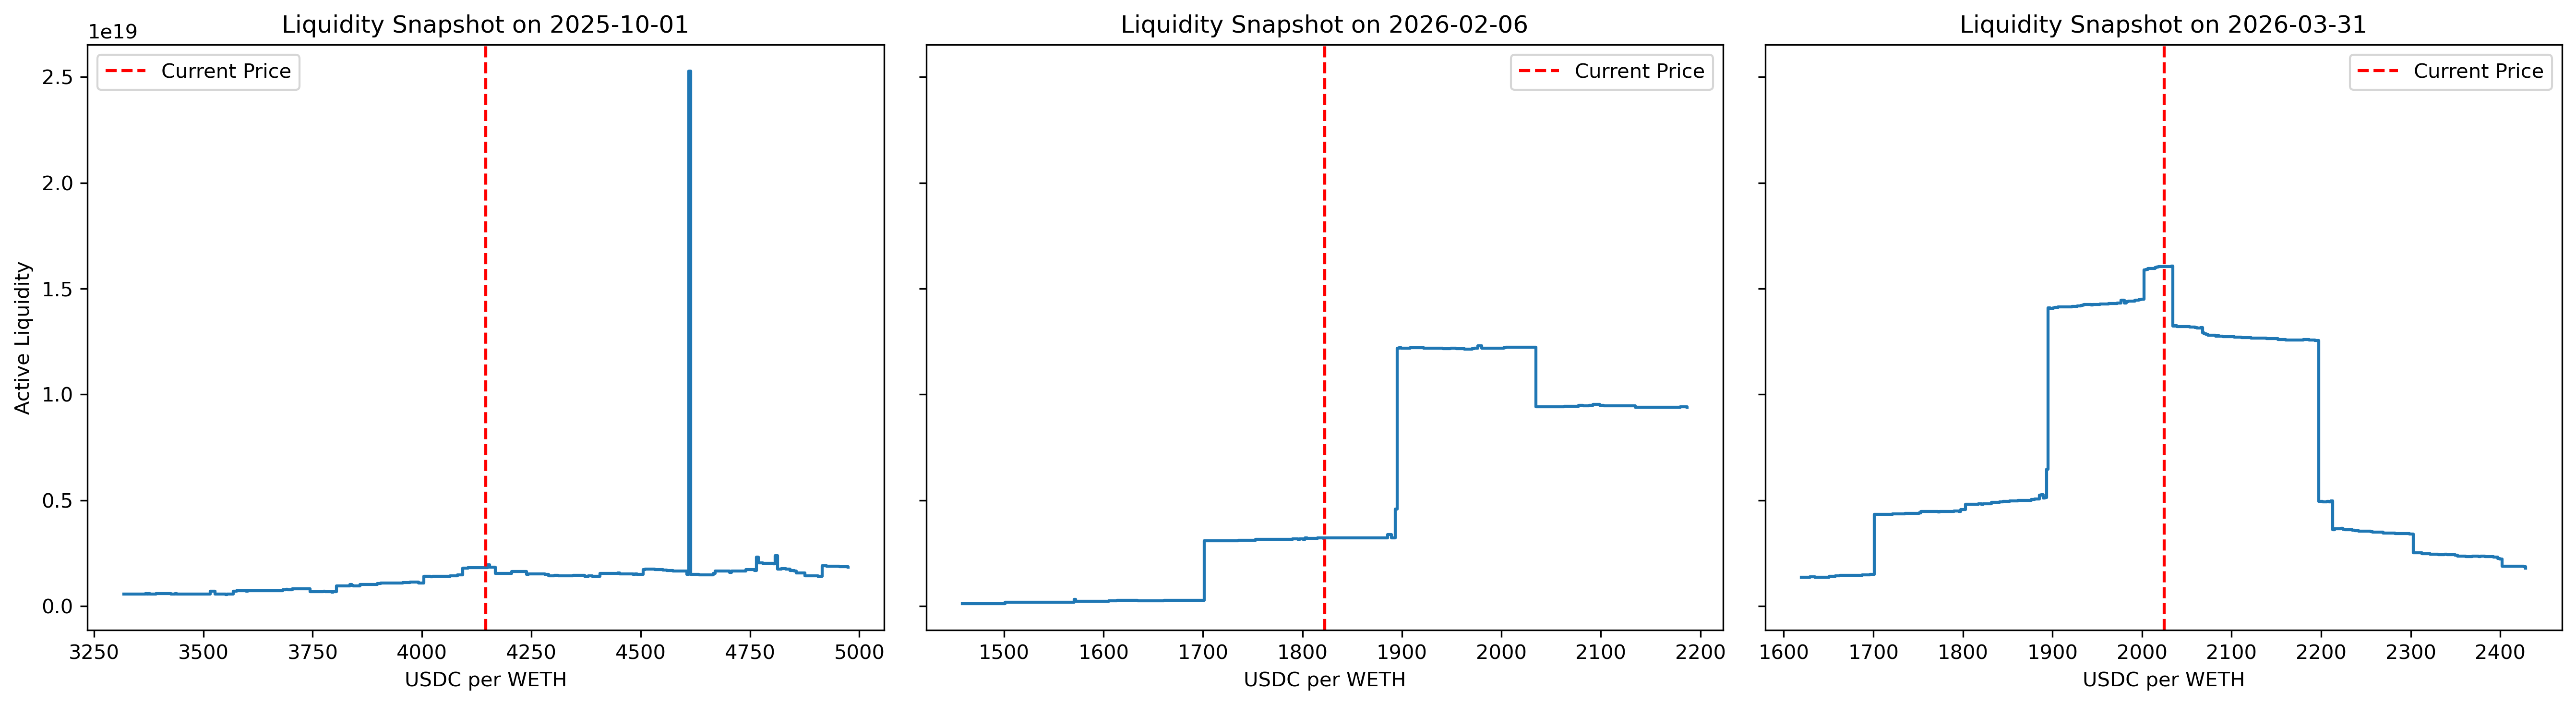
\includegraphics[width=\linewidth]{../data/results/module_2/figures/fig_2_1_liquidity_profiles.png}
    \caption{Fig 2.1 --- Liquidity profiles around the current pool price for three snapshots. The red dashed line marks the current USDC/WETH price.}
    \label{fig:m2-profiles}
\end{figure}

The profiles show that liquidity is not uniformly distributed across prices. At the beginning of the window, when ETH 
traded around \$4,146, most active liquidity was positioned below the current price.  After the price decline into February 
and March, liquidity became much more concentrated around the realized trading range near \$2,000.  The monthly heatmaps in
Figure~\ref{fig:m2-heatmaps} confirm this migration: late-sample liquidity is denser and closer to the current price path than 
in October--December.

These graphs show the liquidity distribution for each snapshot, using the colour as concentration of liquidity, The white line
is the current price. It is a tiled time-series graph, as it shows the heatmap for each day, in monthly groups. We can see that 
the liquidity distribution does migrate towards the current price, thanks to the change in colour of the dark sections at the top and 
bottom of the graph. There is also a clean concentration of liquidity around 2000\$ in all the months. The persistent band around 
\$2{,}000 appears to be a genuine liquidity concentration rather than a plotting artifact: it is present across multiple snapshots 
and is consistent with the underlying initialized-tick liquidity data. This graph also shows the liquidity distribution between roughly 
\$1500 and \$5000. So in the appendix, we show the full price distribution graph using a log price scale \ref{fig:m2-full-price-heatmaps} 
in the appendix \ref{sec:appendix}

\begin{figure}[H]
    \centering
    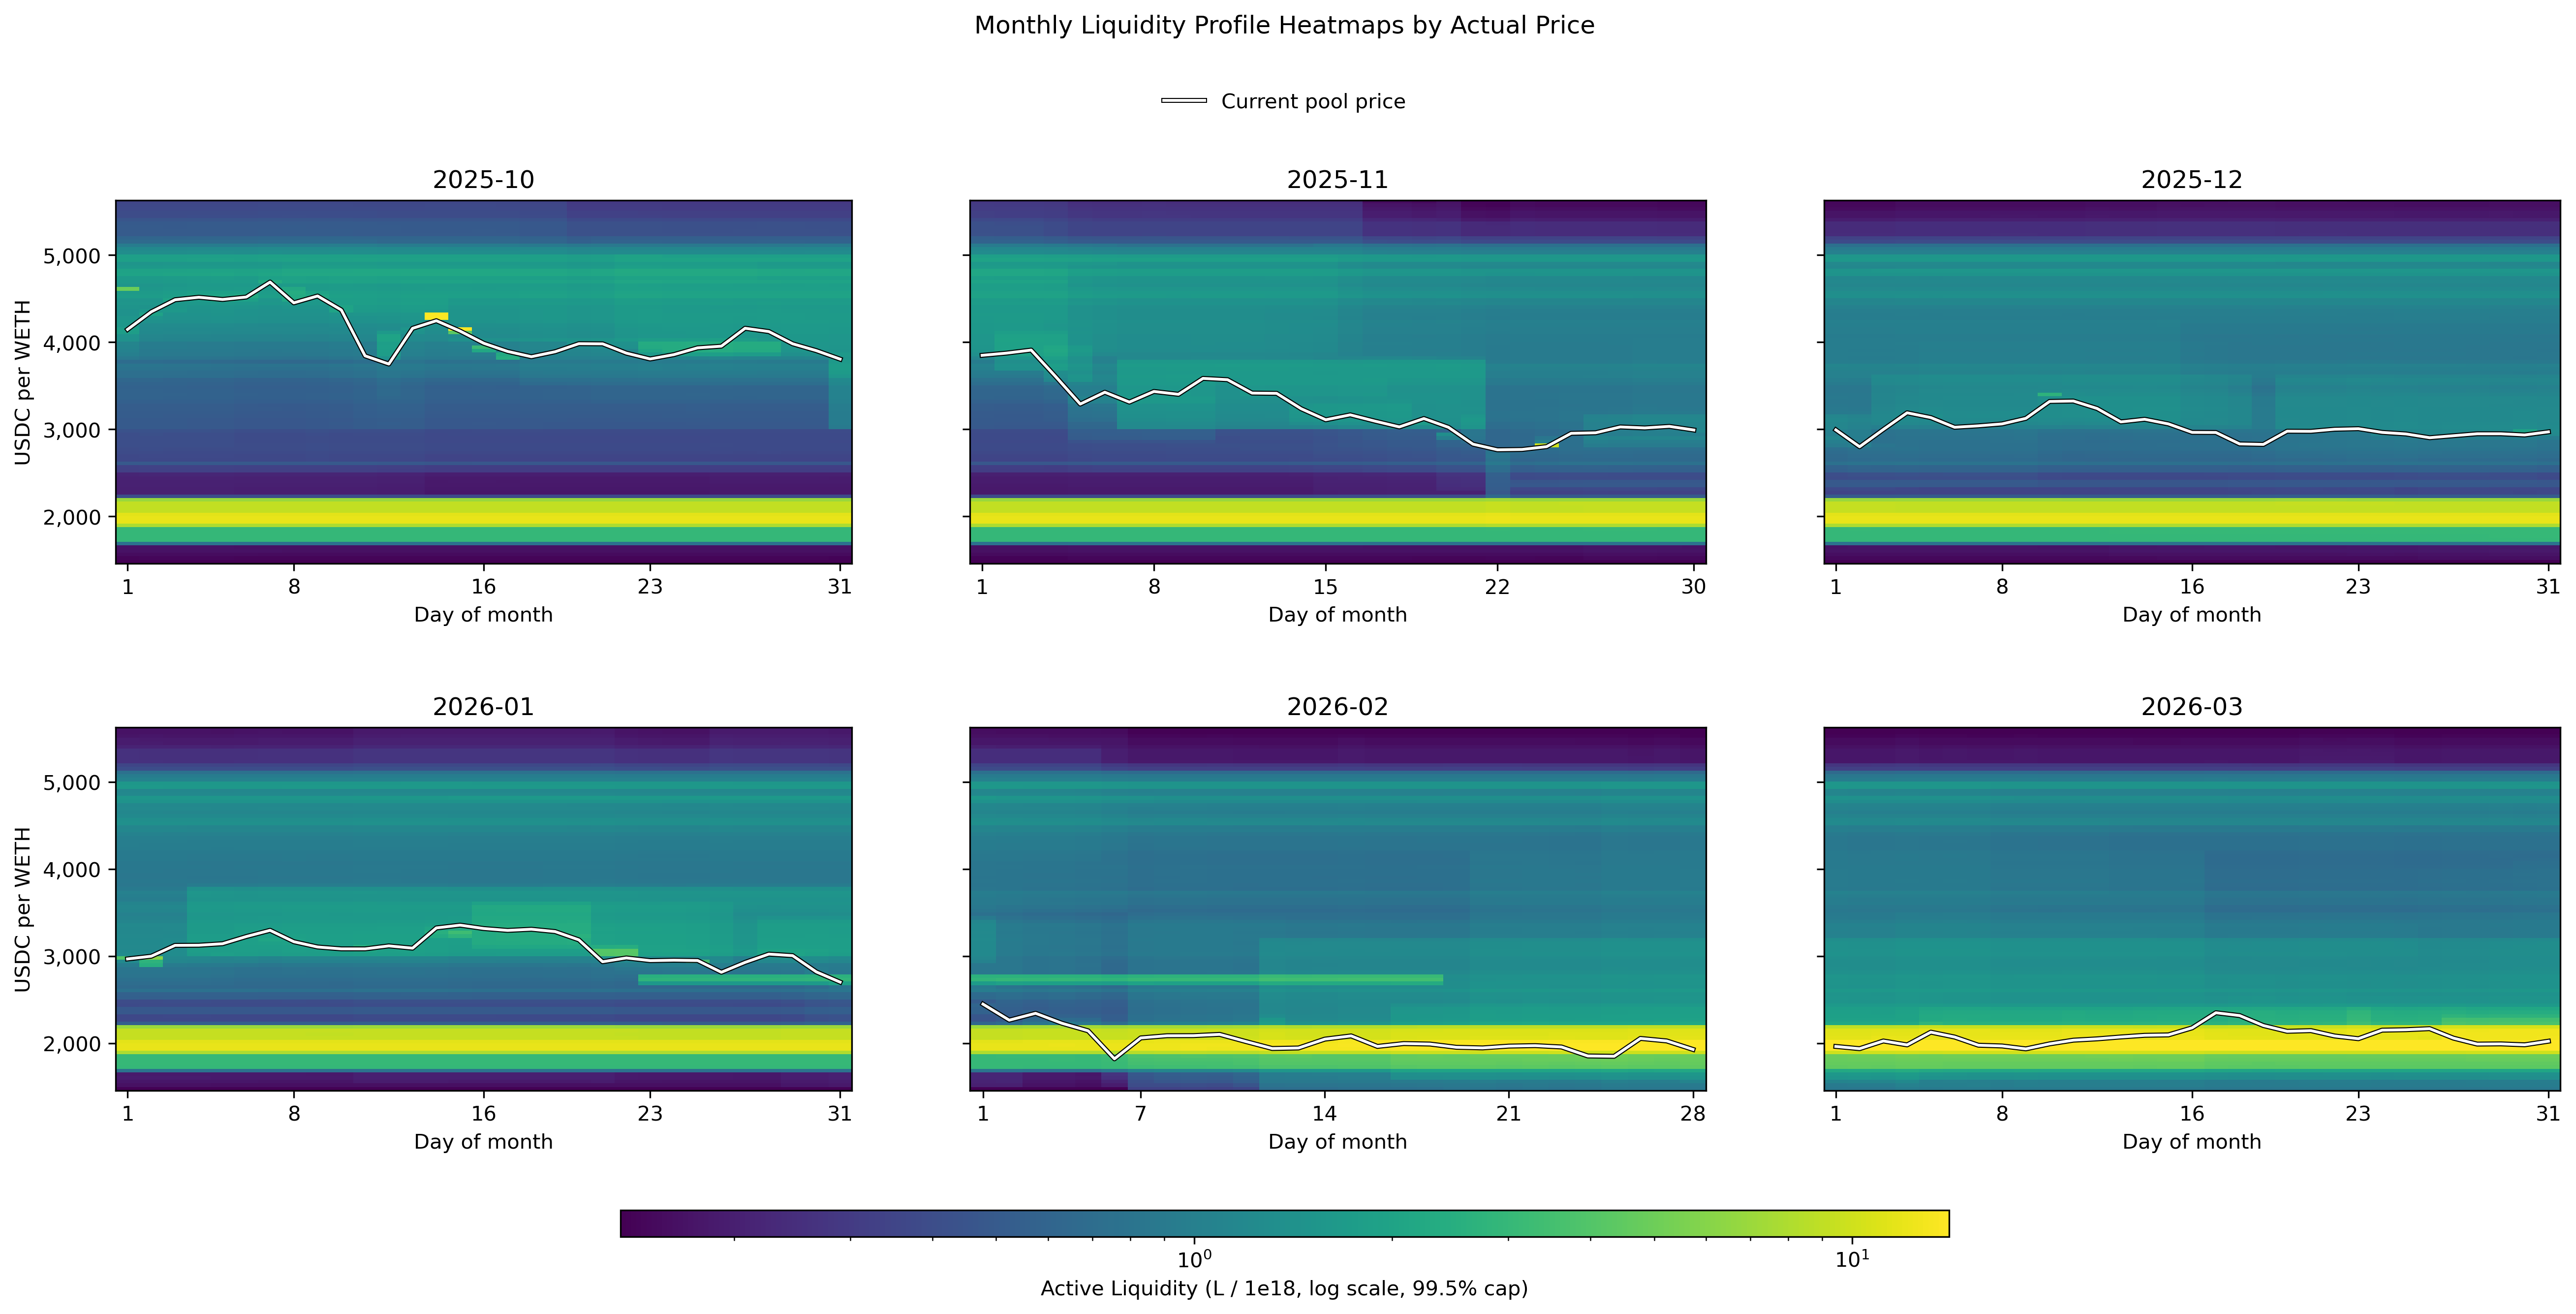
\includegraphics[width=\linewidth]{../data/results/module_2/figures/fig_2_1b_monthly_price_heatmaps.png}
    \caption{Fig 2.1b --- Evolution of the liquidity profile across daily snapshots. Color intensity is active liquidity on a log scale; the white line is the current pool price.}
    \label{fig:m2-heatmaps}
\end{figure}

\subsection{Task 2.2 --- TVL Computation and Decomposition}
\label{subsec:m2-tvl}

Total Value Locked (TVL) is a standard measure of the amount of capital currently deposited in a DeFi protocol. In the context of 
this Uniswap V3 USDC/WETH pool, TVL represents the total dollar value of USDC and WETH supplied by liquidity providers. It gives 
a first indication of the pool’s depth: higher TVL generally means more capital is available to support trades, although in Uniswap 
V3 the location of that liquidity across price ranges is just as important as the total amount.

We compute TVL from the active LP ranges implied by all mint and burn events up to each daily snapshot.  
For a position with liquidity $L$, lower and upper raw square-root prices $s_a<s_b$, and current raw 
square-root price $s$, the Uniswap V3 virtual reserve formulas are
\[
(x,y)=
\begin{cases}
\left(L\dfrac{s_b-s_a}{s_a s_b},\,0\right), & s \leq s_a,\\[1.1em]
\left(L\dfrac{s_b-s}{s s_b},\,L(s-s_a)\right), & s_a<s<s_b,\\[1.1em]
\left(0,\,L(s_b-s_a)\right), & s \geq s_b,
\end{cases}
\]
where $x$ is token0 (USDC raw units) and $y$ is token1 (WETH raw units).  We convert raw units into decimal-adjusted token amounts 
and value each position as
\[
    V = \frac{x}{10^6} + P_{\mathrm{USDC/WETH}}\frac{y}{10^{18}}.
\]
Each position is then classified as in range, above the current USDC/WETH price range, or below it.

\begin{figure}[H]
    \centering
    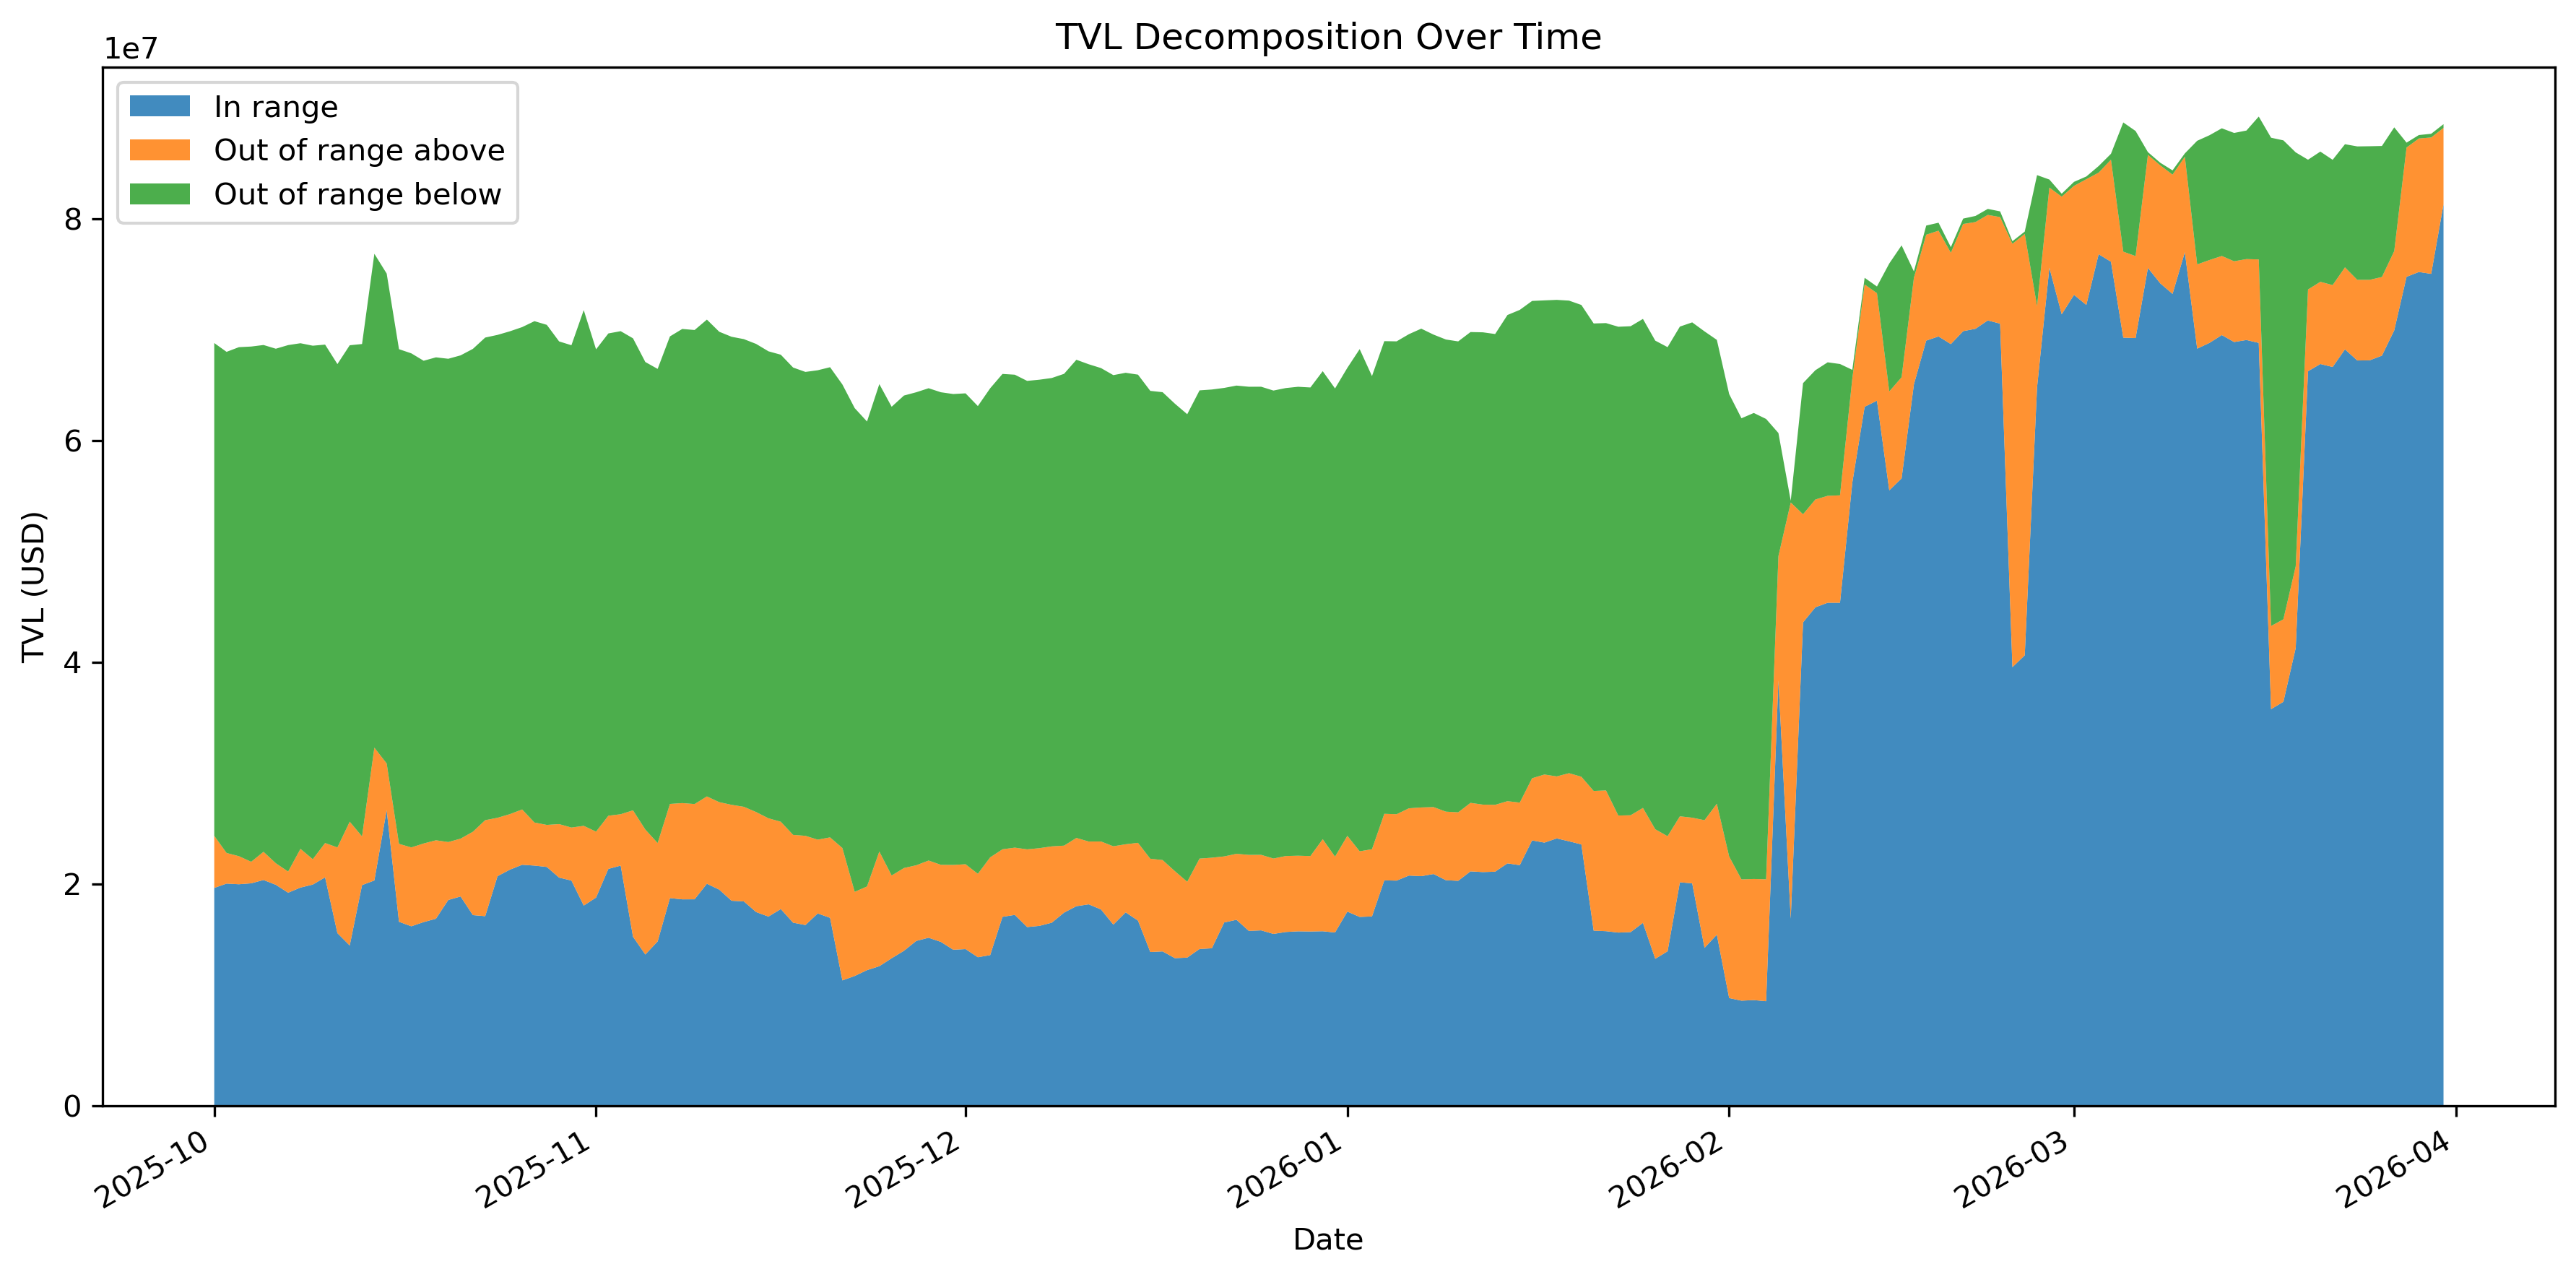
\includegraphics[width=\linewidth]{../data/results/module_2/figures/fig_2_2_tvl_decomposition.png}
    \caption{Fig 2.2 --- TVL decomposition into in-range and out-of-range liquidity across all daily snapshots.}
    \label{fig:m2-tvl}
\end{figure}

Average TVL over the sample is \$71.8 million, with a minimum of \$54.6 million on 6 February 2026 and a maximum of \$89.2 
million on 16 March 2026.  The composition changes sharply over time.  On 1 October 2025, only 28.5\% of TVL was in range, 
while 64.6\% was below range.  On 6 February 2026, in-range TVL was still only 30.9\%, with 68.8\% above range.  By 31 March 
2026, however, 91.8\% of TVL was in range.  This is due for 2 main reasons: the price decline into February and March ment that 
the positions in aeounf 2000\$ mentioned in the previous section became in range, and some migration that followed the price decline. 
The TVL composition is consistent with the liquidity profile visualizations in Figure~\ref{fig:m2-profiles} and the heatmaps in 
Figure~\ref{fig:m2-heatmaps}, which show a clear migration of liquidity towards the current price over time.

\subsection{Task 2.3 --- Liquidity Concentration Metrics}
\label{subsec:m2-concentration}

\subsubsection{Metric A --- In-Range Liquidity Ratio (ILR)}
\label{subsubsec:ilr}

The ILR(k) is defined as the fraction of total active liquidity located within a symmetric price band of ±k\% around the current price.
We will show the ILR for k= 0.1\%, 0.5\%, 1\%, 2\% and 5\%.

We used the formula 
\[
    \mathrm{ILR}(k)_t
    =
    \frac{\sum_i L_{i,t}\mathbf{1}\{P_{i,t}\in[P_t(1-k),P_t(1+k)]\}}
        {\sum_i L_{i,t}},
\]
for $k\in\{0.1\%,0.5\%,1\%,2\%,5\%\}$.  Figure~\ref{fig:m2-ilr} plots all five
series.

\begin{figure}[H]
    \centering
    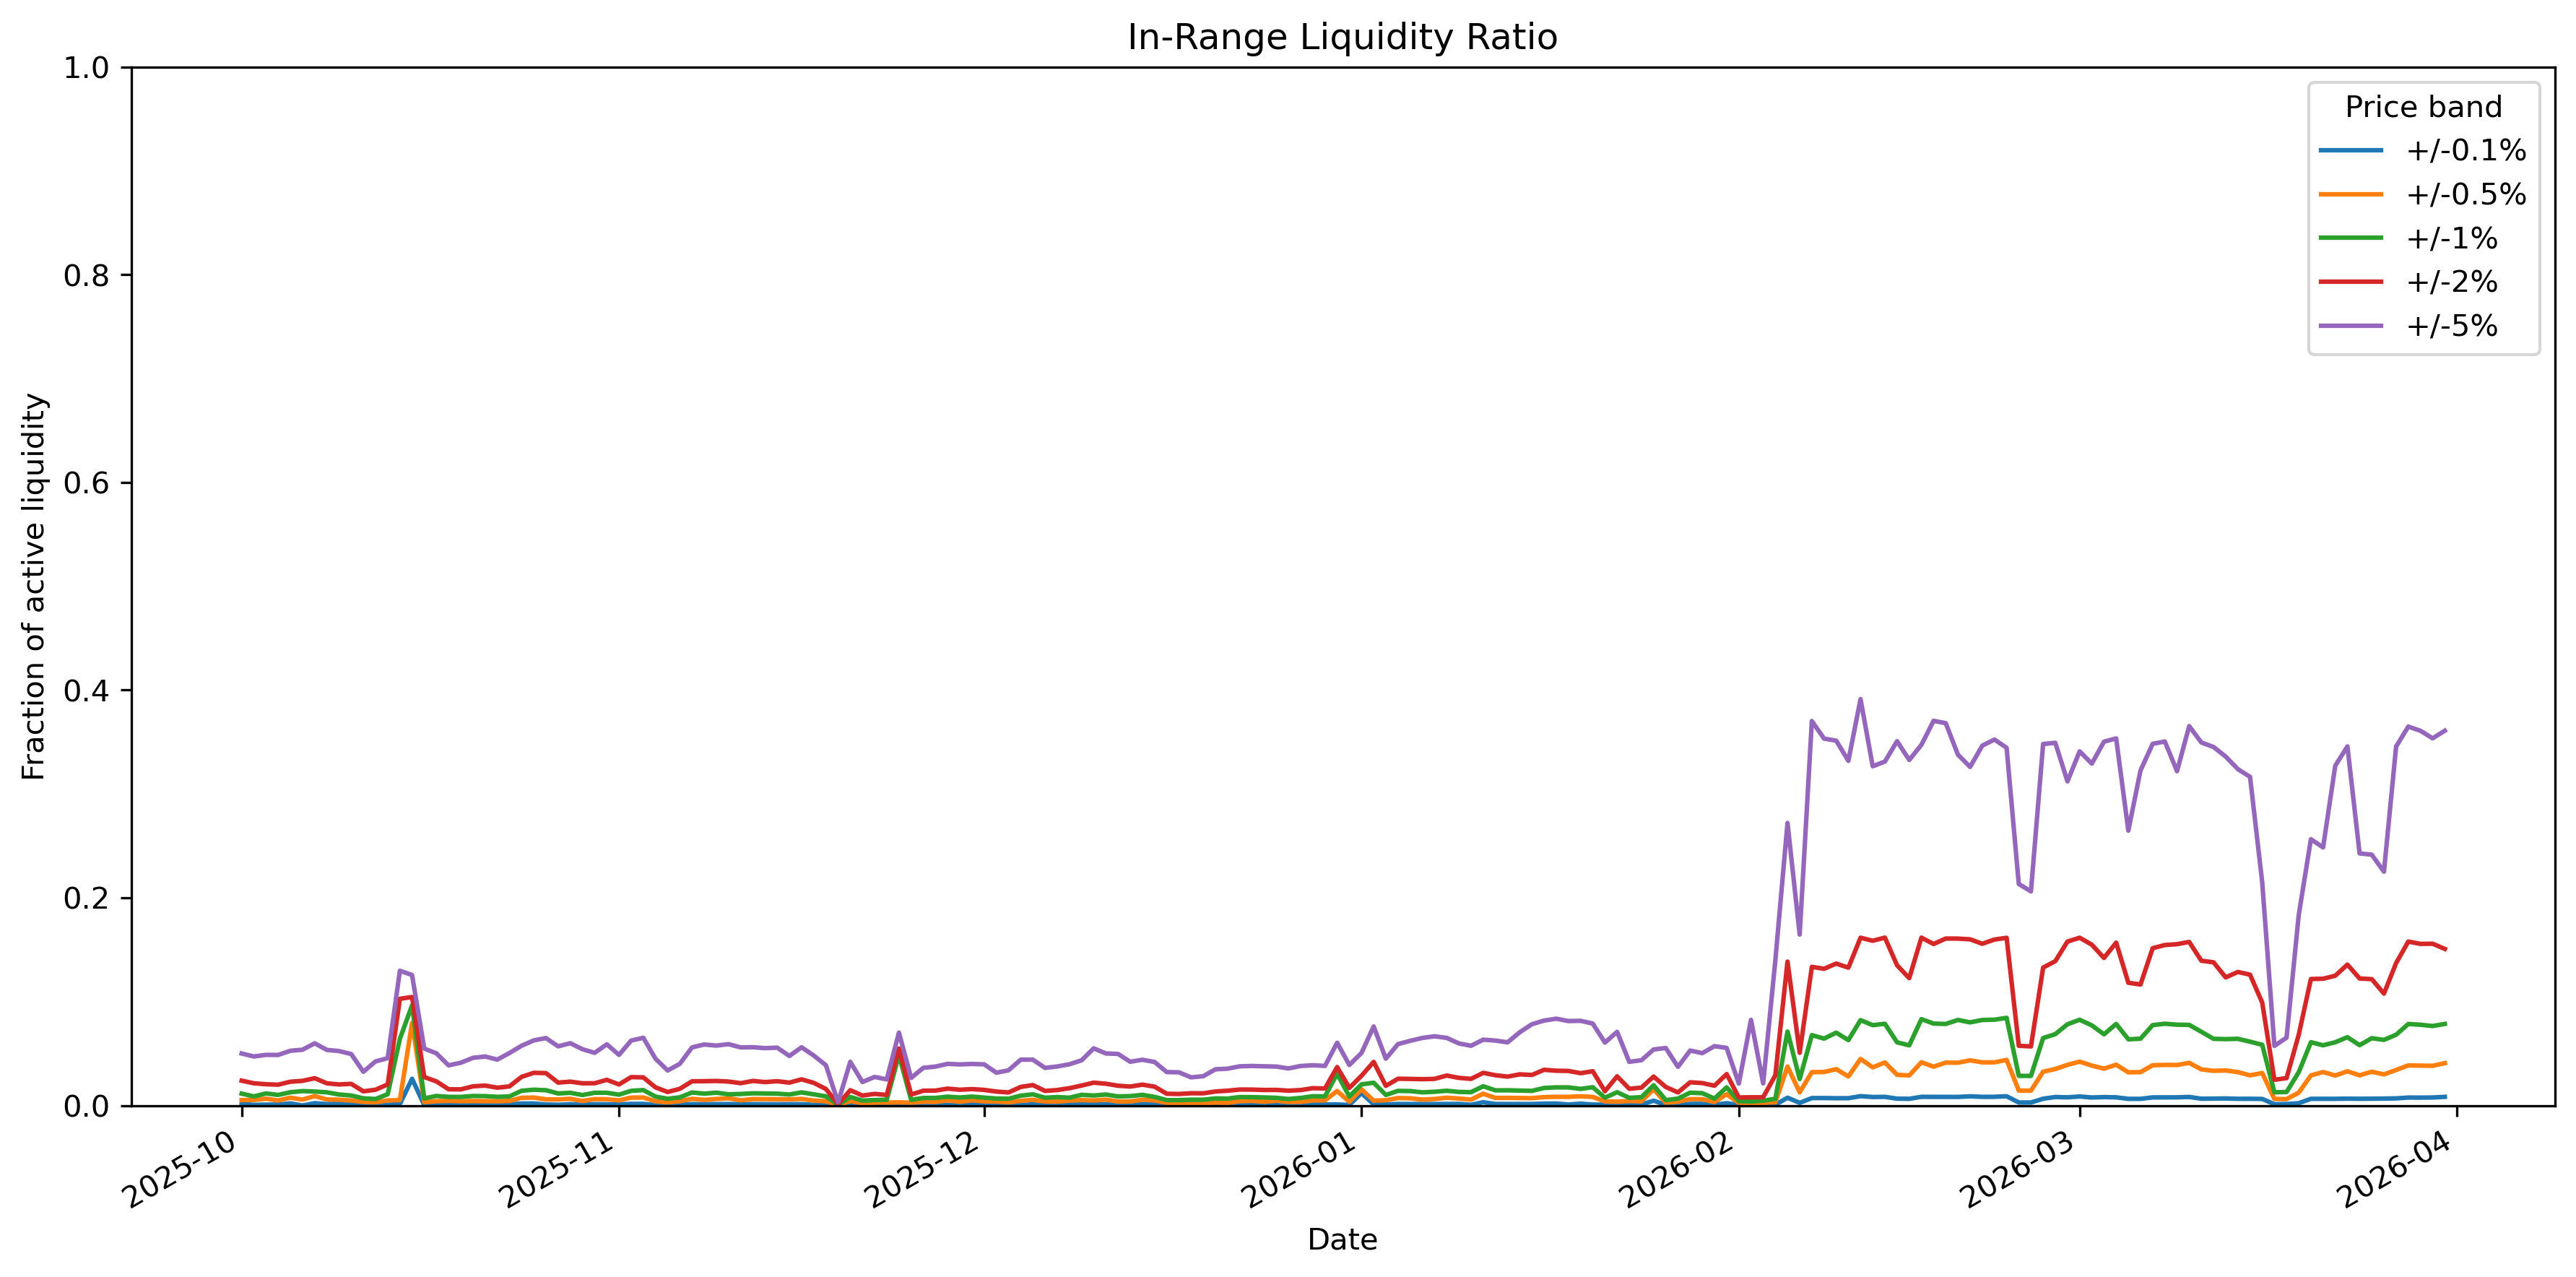
\includegraphics[width=\linewidth]{../data/results/module_2/figures/fig_2_3_ilr_timeseries.png}
    \caption{Fig 2.3.A --- In-range liquidity ratio for symmetric price bands around the current pool price.}
    \label{fig:m2-ilr}
\end{figure}

 The ILR results show that liquidity near the marginal price increased
substantially over the sample.  The 5\% ILR averaged 12.9\%, but rose from
5.0\% on 1 October 2025 to 36.1\% on 31 March 2026.  The 1\% ILR rose from
1.14\% to 7.85\% over the same dates.  This supports the visual evidence that
liquidity became more tightly centered around the realized trading range in
February and March.

\subsubsection{Metric B ---Liquidity Herfindahl-Hirschman Index (L-HHI)}
\label{subsubsec:lhhi}

The L-HHI is the sum of squared liquidity shares across all initialised ticks,
\[
    \mathrm{HHI}=\sum_i \left(\frac{L_i}{\sum_j L_j}\right)^2.
\]
An L-HHI close to 1 indicates liquidity concentrated in very few ticks; a value close
to 0 indicates near-uniform distribution.

We computed the L-HHI for each daily snapshot using the formula
\[
    \mathrm{LHHI}_t
    =
    \sum_i
    \left(
        \frac{L^{gross}_{i,t}}{\sum_j L^{gross}_{j,t}}
    \right)^2.
\]
We overlay L-HHI with the ETH price in Figure~\ref{fig:m2-lhhi}.

\begin{figure}[H]
    \centering
    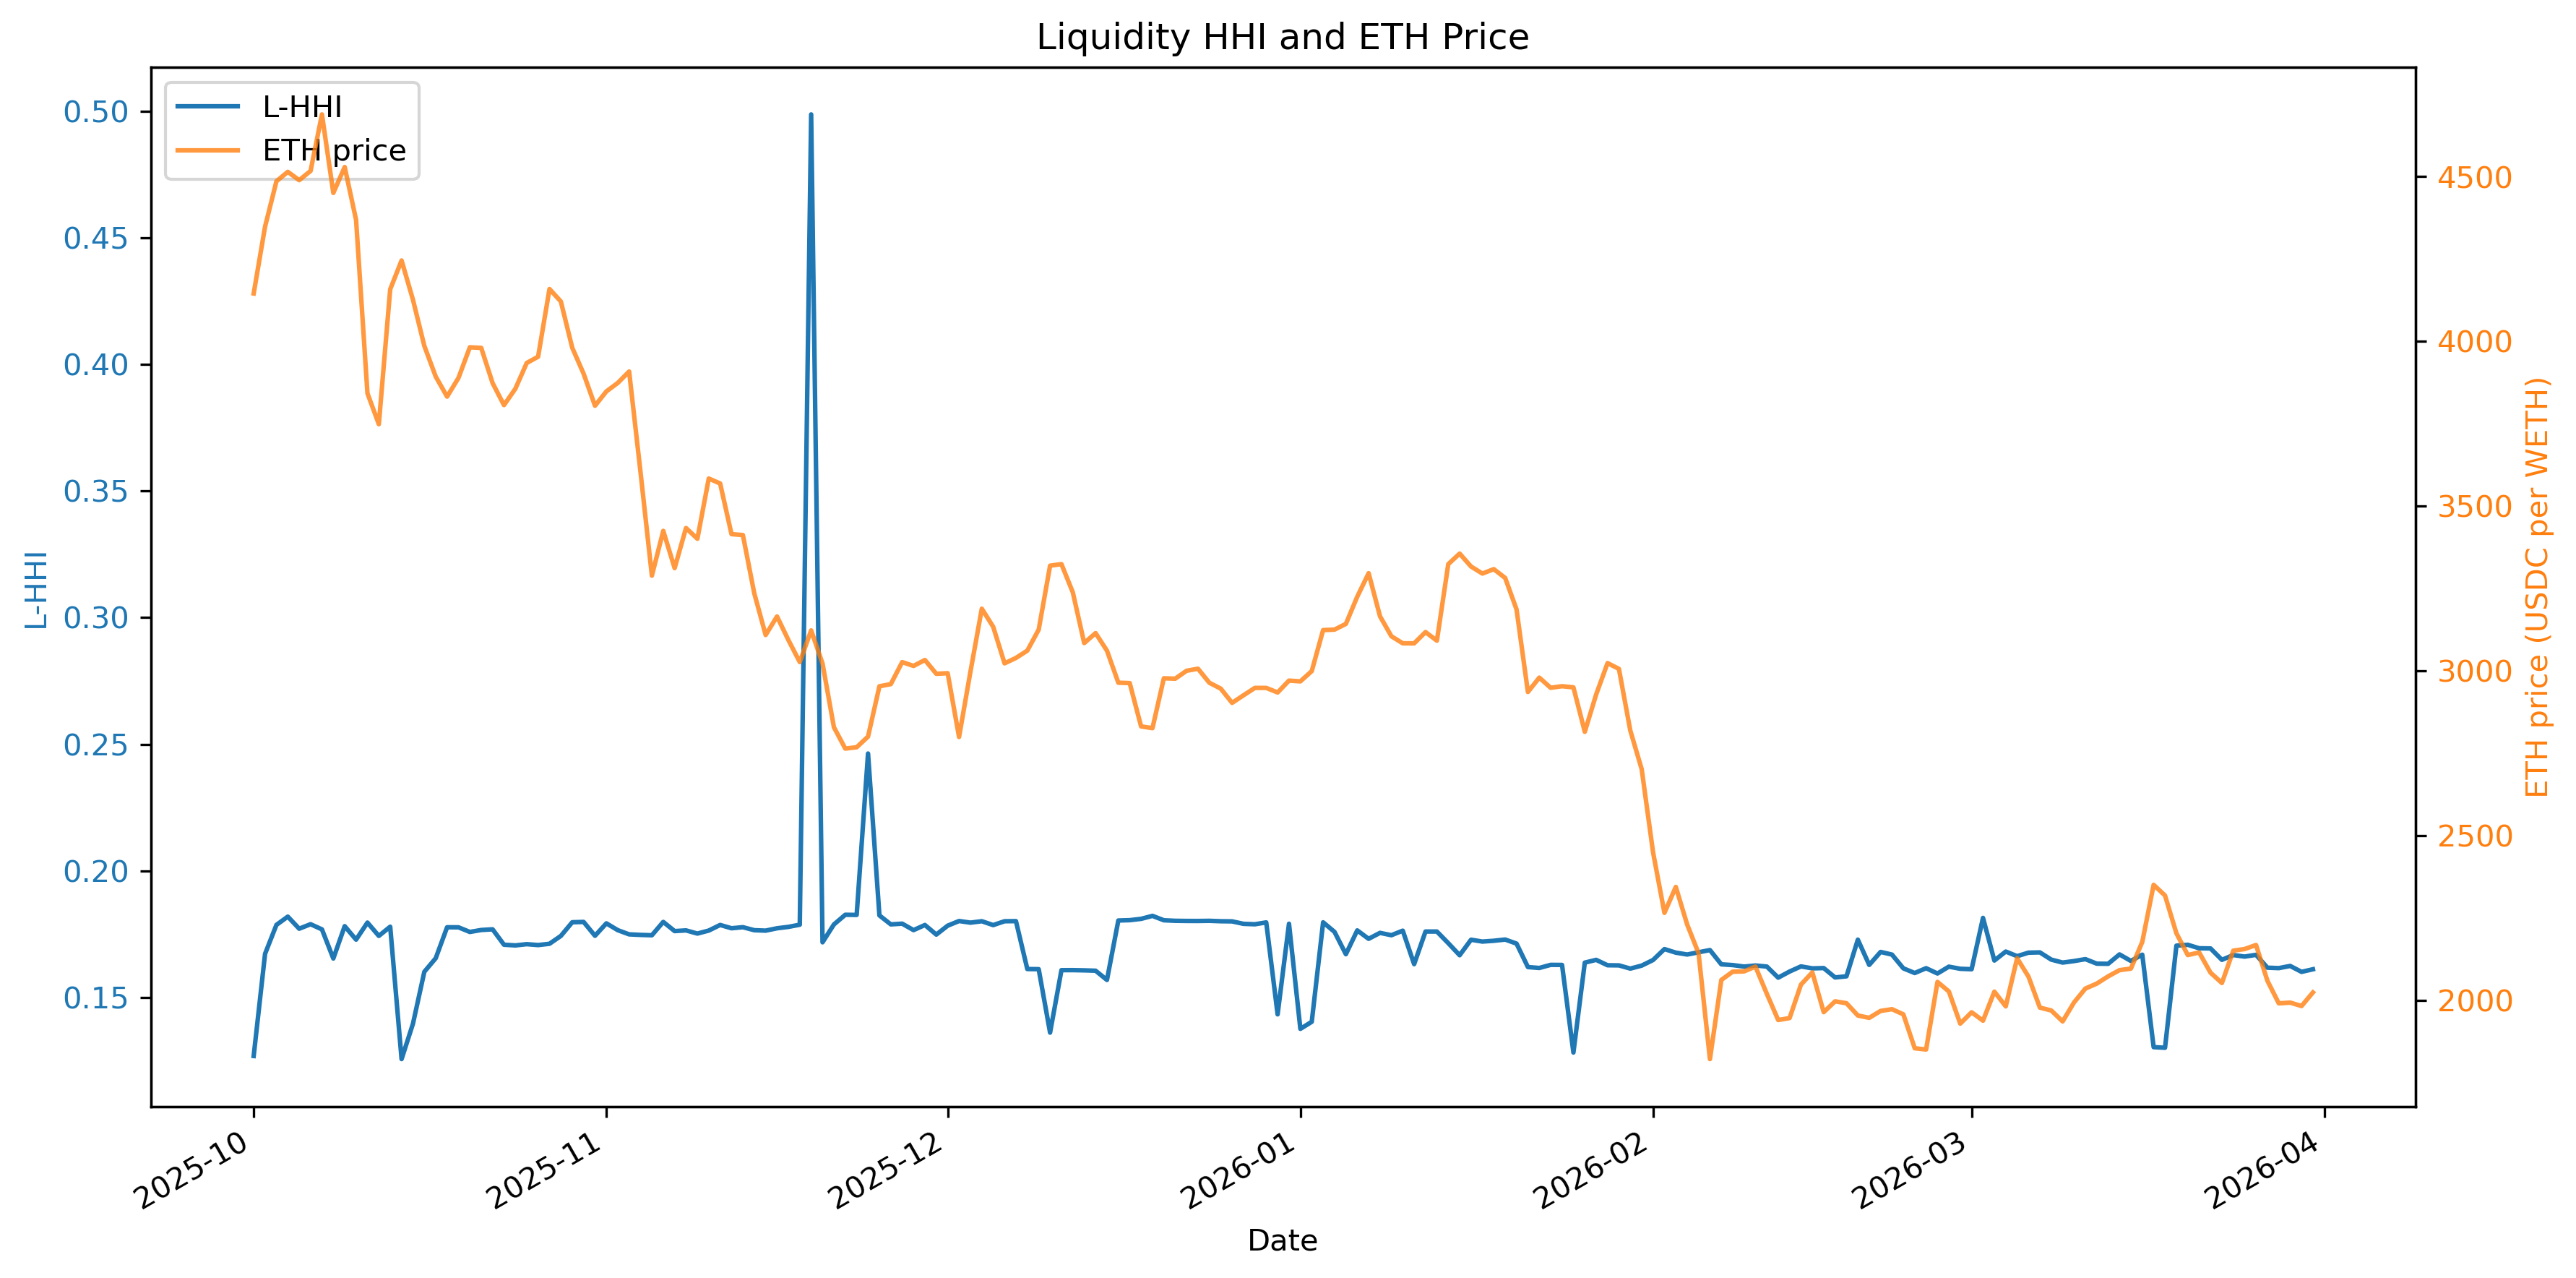
\includegraphics[width=\linewidth]{../data/results/module_2/figures/fig_2_3_lhhi_eth_price.png}
    \caption{Fig 2.3.B --- Liquidity HHI and ETH price.}
    \label{fig:m2-lhhi}
\end{figure}

The average L-HHI is 0.171, with a minimum of 0.126 and a maximum of 0.499. Unlike ILR, L-HHI does not move 
mechanically with the ETH price: the correlation between price and L-HHI is only 0.12.  This is because L-HHI 
measures concentration across initialized ticks globally, whereas ILR measures how much liquidity is close to 
the current price.  Together, the two metrics show that late-sample execution liquidity improved mainly because 
LPs moved liquidity toward the current price, not because the entire tick distribution became uniform.
